\section{Vorbereitung}
Vor der Durchführung ist sich anhand der Literatur über die Dichte $\rho$, die spezifische Wärme c und die Wärmeleitfähigkeit $\kappa$ für Aluminium, Messing und Edelstahl zu informieren.
Diese Werte wurden  in Tabelle (\ref{tab:literaturwerte}) zusammengetragen:

\begin{table}
\centering
\begin{tabular}{c c c c }
\toprule
{Material} &{$ \rho \mathbin{/} \si[per-mode=fraction]{\kilo\gram\per\cubic\meter} $} & {c $ \mathbin{/} \si[per-mode=fraction]{\joule\per\kilo\gram\per\kelvin} $} & {$ \kappa \mathbin{/} \si[per-mode=fraction]{\watt\per\meter\per\kelvin} $} \\
\midrule
Aluminium & 2700 & 896 & 221 \\
Messing   & 8730 & 384 & 142 \\
Edelstahl & 8000 & 500 & 21  \\
\bottomrule
\end{tabular}
\caption{Literaturwerte}
\label{tab:literaturwerte}
\end{table}

\newpage
\section{Versuchsaufbau}

\begin{figure}
            \centering
               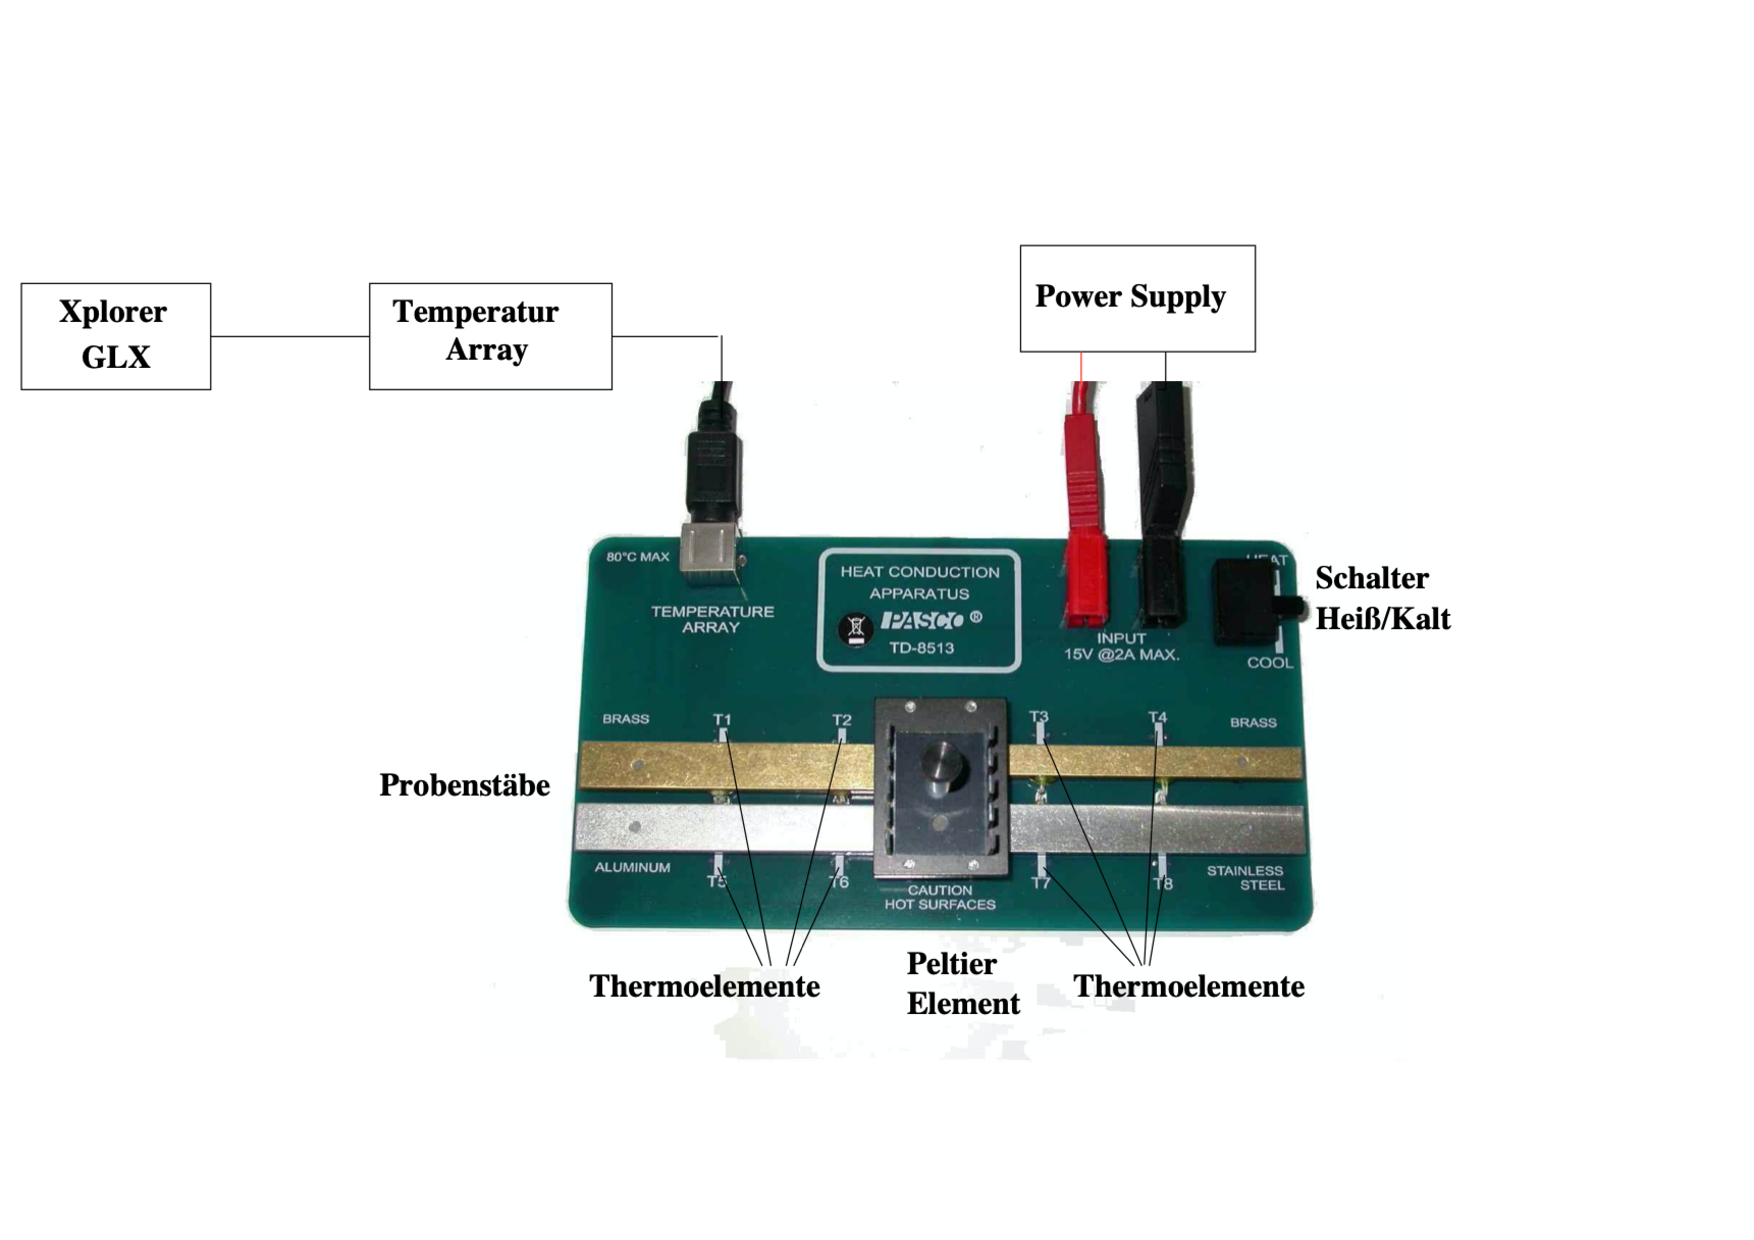
\includegraphics[height=9cm]{V204_aufbau.pdf}
               \caption{Prinzipieller Aufbau.}
               \label{fig:aufbauwaermeleitung}
        \end{figure}

\noindent
In der Abbildung (\ref{fig:aufbauwaermeleitung}) ist das Experiment zur Bestimmung der Wärmeleitfähigkeit zu sehen.
Auf der Grundplatte befinden sich vier rechteckige Probenstäbe unterschiedlicher Art.
Darunter einer aus Aluminium, einer aus Edelstahl und zwei unterschiedlicher Breite aus Messing.
Die Probenstäbe können mithilfe des Peltierelements durch betätigen des Schalters abwechselnd gekühlt oder erhitzt werden.
An das Peltierelement wird für die statische Methode eine Spannung von $U_P=5V$ und für die dynamische Methode eine Spannung von $U_P=8V$ angelegt.
Pro Stab gibt es zwei Thermoelemente mit denen die Temperatur an der jeweiligen Stelle gemessen werden kann.
Die Temperaturen und Temperaturverläufe werden über ein 'Temperatur Array' an einen Datenlogger (Xplorer GLX) weitergegeben und können dort eingesehen, bearbeitet und graphisch dargestellt werden.
Außerdem wurde seperat eine Stoppuhr zur Verfügung gestellt.
Diese Daten (\ref{tab:probenstaebe}) für die Probenstäbe wurden bereitgestellt:

\begin{table}
\centering
\begin{tabular}{c c c c }
\toprule
{Material} & Abmessungen $\mathbin{/} \si{\centi\meter}$ &{$ \rho \mathbin{/} \si[per-mode=fraction]{\kilo\gram\per\cubic\meter} $} & {c $ \mathbin{/} \si[per-mode=fraction]{\joule\per\kilo\gram\per\kelvin} $} \\
\midrule
Messing (breit)   & 9 x 1.2 x 0.4 & 8520 & 385 \\
Messing (schmal)  & 9 x 0.7 x 0.4 & 8520 & 385 \\
Aluminium (breit) & 9 x 1.2 x 0.4 & 2800 & 830 \\
Edelstahl (breit) & 9 x 1.2 x 0.4 & 8000 & 400 \\
\bottomrule
\end{tabular}
\caption{Daten der Probenstäbe}
\label{tab:probenstaebe}
\end{table}

\section{Versuchsdurchführung}
Vorerst wird die Verkabelung überprüft.                                                                                                                                                                                    
Der Abstand $\Delta x$ der Messstellen zwischen den Thermoelementen wird mithilfe eines Lineals mit der Messunsicherheit $\Delta s = \pm 0.05 \si{\centi\meter}$ gemessen.

\begin{equation}
_\text{Diese Abstände wurden gemessen}
\label{eqn:abstand}
\end{equation}

\begin{align*}
    \Delta x_\text{T1T2} &= 2.9 \si{\centi\meter} \\
    \Delta x_\text{T3T4} &= 3.0 \si{\centi\meter} \\
    \Delta x_\text{T5T6} &= 3.1 \si{\centi\meter} \\
    \Delta x_\text{T7T8} &= 3.1 \si{\centi\meter} 
\end{align*}

\noindent Es werden Messungen verschiedener Methoden durchgeführt.

\subsection{Statische Methode}
Bei der statischen Methode wird die Temperatur als Funktion der Zeit an den zwei Messstellen pro Stab gemessen, um über den zeitlichen Temperaturverlauf die Wärmeleitfähigkeit zu bestimmen.

\noindent Hierzu wird zunächst die Abtastrate $\Delta t_\text{GLX}$ am Datenlogger auf 5s gesetzt.
Unter Menüpunkt Digital werden die Temperaturen aller acht Sensoren eingesehen.
Die Isolierung wird auf die Stäbe gelegt.
Nun wird bei maximalem Strom eine Spannung von 5V angelegt und der Schalter wird von 'COOL' auf 'HEAT' umgelegt,
während die Messung auf dem Xplorer GLX gestartet wird.
Die Messung wird beendet, wenn die Temperatur des Thermoelements T7 45 Grad anzeigt.
Die Messergebnisse werden mit einem zur Verfügung gestellten Stick zur Weiterverarbeitung der Daten gesichert.
Die Isolierung wird abgenommen und der Schalter wird auf 'COOL' umgelegt.
Die Probenstäbe werden so lange gekühlt, bis jedes Thermoelement eine Temperatur von 30 Grad oder kälter hat.
Um längeren Wartezeiten vorzubeugen wurde die Platine mit einer nicht benutzten Platine ausgetauscht.

\newpage
\subsection{Dynamische Methode}
Bei der Angström Methode wird die Wärmeleitfähigkeit aus der Ausbreitungsgeschwindigkeit der Temperaturwelle berechnet,
die sich ergibt, wenn ein Probenstab periodisch geheizt wird.

\noindent Dazu wird die Abtastrate $\Delta t_\text{GLX}$ am Datenlogger auf 2s gesetzt.
Im Unterverzeichnis Digital wird überprüft, ob die Probenstäbe an jeder Messstelle hinreichend abgekühlt sind (30 Grad oder kälter).
Die Isolierung wird auf die Stäbe gelegt und die Messung wird gestartet, sobald eine Spannung von 8V angelegt wird.
Die Probenstäbe werden daraufhin mit einer Periode von 80s geheizt.
Der Schiebeschalter wird zu Beginn der Messung 40s auf 'HEAT' gestellt und danach 40s auf 'COOL' gestellt.
Als Hilfsmittel wird hier die Stoppuhr verwendet.
Die Messung wird nach 11 Perioden beendet und die Daten per Stick gesichert.
Die Isolierung wird abgenommen und der Schalter bleibt auf 'COOL'.

\noindent Nachdem die Platine wieder aufgrund der langen Abkühlzeit der Probenstäbe ausgetauscht wurde, wird eine neue Messung gestartet.
Dabei wird der eben beschriebene Vorgang wiederholt, allerdings mit einer Periode von 200s.
Dafür werden die Stäbe 100s erhitzt und anschließend 100s gekühlt.
Hierfür wird wieder eine Stoppuhr verwendet.
Die Messung wird beendet, wenn eins der Thermoelemente eine Temperatur von über 80 Grad erreicht, was nach 4 Perioden der Fall war. 
Die Daten werden gesichert und alle Gerätschaften abgeschaltet, sobald die Stäbe abgekühlt sind.
Alle Messvorgänge sind nun beendet.
